\subsubsection{Terminology}
\label{sub:sn_terminology}

As with deep learning, social network terminology is sometimes used in confusing
ways.
This subsection aims to introduce concepts regarding social networks, as well
as describe the growing influence of social media on companies.
Firstly, the term \textit{social network} is defined, before structural
properties are explained (ch.~\ref{sub:sn_social_networks}).
The second part of this section focuses on \textit{social media}, especially
practical implications for organizations (ch.~\ref{sub:sn_social_media}).

\paragraph{Social networks}
\label{sub:sn_social_networks}

In order to examine social network structure and properties, the term first
has to be defined.
Wassermann \& Faust (1994) explicate that `a social network consists of a finite
set or sets of actors and the relation or relations defined of them'~\footcite[20]{Wasserman1994}.
Here, an \textit{actor} can be any social entity, e.g, people, groups, countries or
organizations.
\textit{Relations} are then batches of ties between these entities, e.g., resource
transfers, associations or interactions~\footcite{Wasserman1994}.
With this basic definition set, the next two paragraphs focus on structure and
properties of social networks.

\paragraph{Structure}

Social networks can be visualized using graphs, where actors serve as nodes
and lines represent relations between these actors.
Thus, the network consists of a set of nodes $N = \{n_1, n_2, \cdots, n_g\}$ and
a set of lines $L = \{l_1, l_2, \cdots, l_L\}$~\footcite{Wasserman1994}.

\begin{figure}[h]
  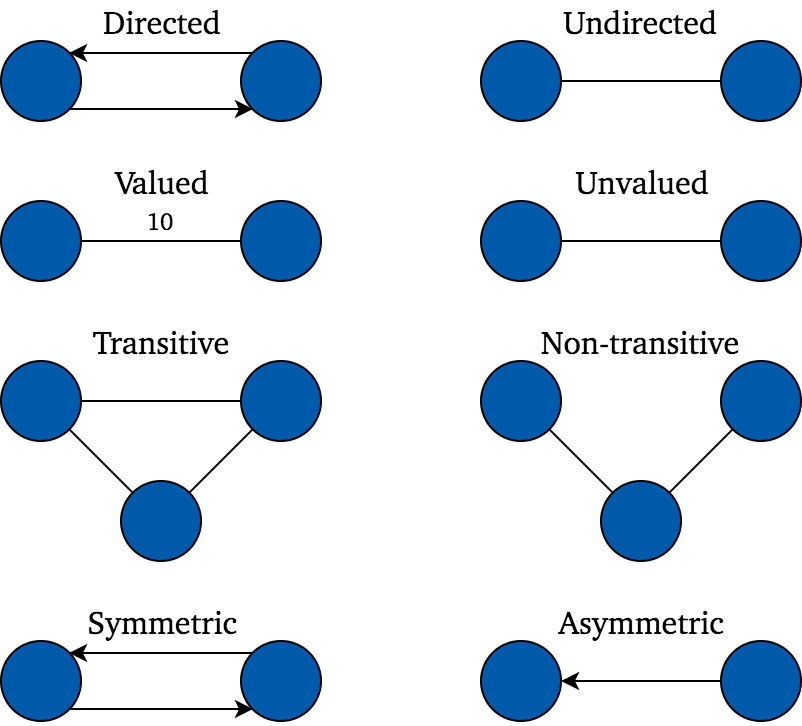
\includegraphics[height=8cm]{img/relation_properties}
  \caption{Relation properties in social networks}
\label{fig:tie_properties}
\end{figure}

Relations between actors can have several properties, as denoted in Fig.~\ref{fig:tie_properties}.
A first distinction has to be made between directed and undirected relations,
a property that also determines the directionality of the underlying graph.
An example for a directed relation would be resource transfers, an undirected
relation could be exemplified by marital relationships.
Relations can also be split into valued and unvalued types.
The attached value can stand for several properties, e.g., interaction intensity
between two actors.
Transitive relations occur when actor triples are connected to each other.
More intuitively, transitivity means that two related actors of an actor $n$ are
also related.
The final property exemplified in Fig.~\ref{fig:tie_properties} is symmetry which
is always given in undirected networks.
For undirected networks, symmetry refers to the existence of a relation from
$n_i$ to $n_j$, if there is a relation in the opposite direction~\footcite{Wasserman1994}.

\paragraph{Properties}

Social network analysis is a research area which examines dynamics in social
networks.
A central research question is the identification of important actors within
a network.
Important actors are also referred to as prestigious or prominent, where importance
represents the extent to which these actors are involved with others.
Here, involvement means being the sender or recipient of interactions in the
network.
A common measure for actor prominence is \textit{centrality}, which delivers
several characteristic numbers for measuring activity and location of an actor~\ref{Wasserman1994}.
Observations in social network analysis contain the \textit{small world problem},
which is related to the probability of two random actors in a network being
connected to each other.
Formulated differently, the problem also comprises the question how many
mutual acquaintances are needed to form a path between these random actors.
Experiments lead to the conclusion that the distance between two actors in
a network is surprisingly low~\footcite{Travers1969}.
This gives way to observations that stress the importance of so-called
\textit{weak ties}, i.e., relations between actors that are less intense and
intimate, but serve significant roles in information diffusion~\footcite{Granovetter1973}.

\begin{figure}[h]
  
\includegraphics[height=6cm]{img/power_law_linkages}
  \caption[Power Law Distribution of Node Linkages]{Power Law Distribution of Node Linkages~\footcite{Barabasi2003}}
\label{fig:power_law}
\end{figure}

In addition to the small world phenomenon, many social networks are observed to
be \textit{scale-free}.
Scale freedom denotes that few actors have a very high number and most actors 
a low number of connections.
Highly connected nodes are referred to as \textit{hubs}.
A power law distribution can be observed in scale-free networks, i.e., the
probability for an actor to have exactly $k$ connections is given by $k^{-n}$
where $n$ is approximately 2~\footcite{Barabasi2003}.
Fig.~\ref{fig:power_law} shows the power law distribution of node linkages both
on a regular and log-scale.

\paragraph{Social media}
\label{sub:sn_social_media}

The terms social network and social media are often used interchangeably, though
they generally refer to distinct matters.
Social media can be described as `a group of Internet-based applications that
build on the ideological and technological foundations of Web 2.0, and that allow
the creation and exchange of User Generated Content'~\footcite[61]{Kaplan2010}.
\textit{Web 2.0} refers to technologies like \textit{Flash}, \textit{RSS} and 
\textit{AJAX} that first enabled collaboration on the internet, e.g., via blogs
or wiki pages.
Examples for social media platforms are \textit{Facebook} (social network), 
\textit{Twitter} (microblogging) or \textit{YouTube} (video platform).
Upcoming of social media platforms brings practical challenges for organizations,
since they enable both direct communication with the customer, as well as
communication between customers.
Contents and frequency of the latter are mostly out of managerial control~\footcite{Mangold2009}.
Nowadays, most companies maintain social media profiles as part of their
marketing strategy.
Research has created guidelines for corporate use of social media and stressed the
importance of community building around products of a company~\footcite{Culnan2010}.
Here, tracking the return of social media investments often requires engagement
statistics, e.g., number of followers, visits or replies, as well as community
sentiment~\footcite{Hoffman2010}.
Attributes of social media marketing have been shown to have positive effects
on purchase intention, e.g., for luxury fashion brands~\footcite{Kim2012}.

Twitter has been listed as an example social media platform.
The concluding section of the background chapter will explain terminology
and properties related to Twitter in more detail.
